%!TEX root = ../dokumentation.tex

\chapter{Bedienung der Anwendung}

Abbildung \ref{Bild1} zeigt die Anwendung nach dem Start. Zu sehen ist eine Liste von Bilder, die der App entweder durch das Aufnehmen eines Fotos oder das Laden eines Bildes aus der Galerie hinzugefügt wurde. Links neben dem Foto werden ein Titel, das Datum und die Uhrzeit, an dem das Bild aufgenommen wurde, angezeigt.

\vspace*{\lineskip}
\begin{wrapfigure}[10]{R}{5cm}
\label{Bild1}
\centering
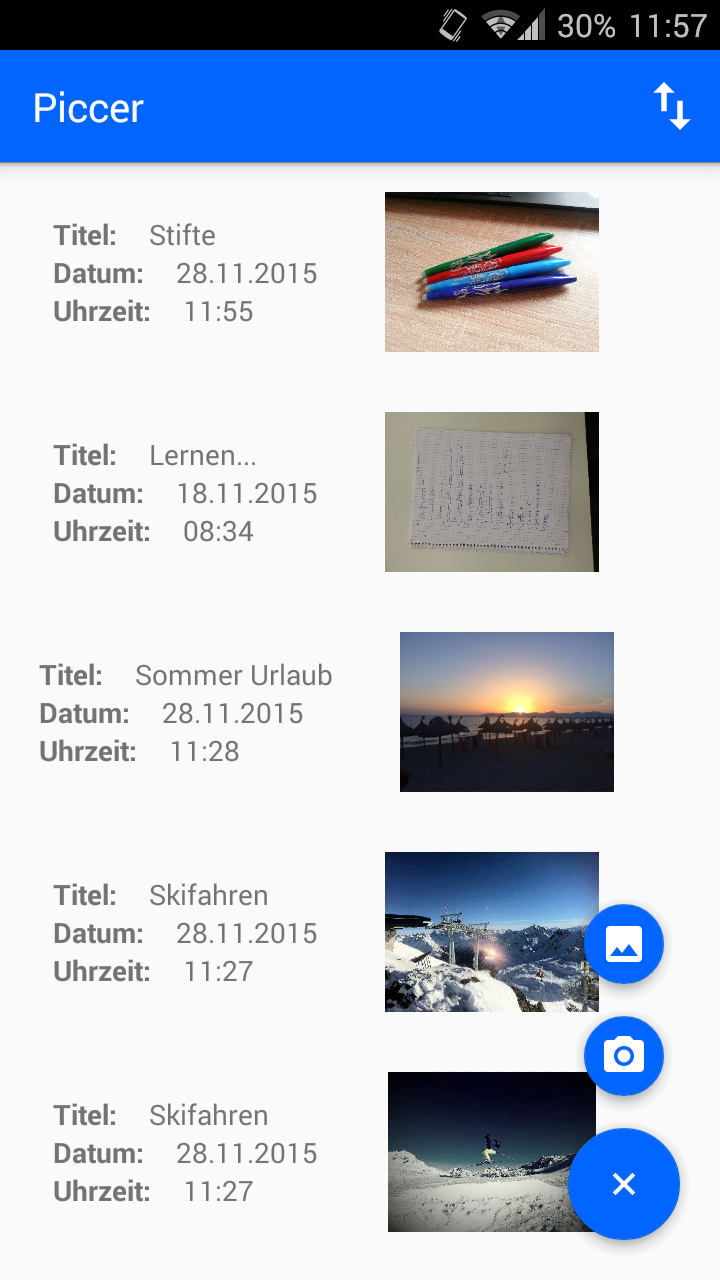
\includegraphics[width=0.2\textwidth]{images/bild_1}
\caption{Bild 1}
\end{wrapfigure}


Wird ein Bild aus der Galerie geladen und es liegt ein Datum vor, wann es aufgenommen wurde, so zeigt \enquote{Piccer} dieses Datum an. Falls es nicht möglich ist, ein solches Datum aus der Datei auszulesen, wird das Datum gesetzt, wann das Bild hinzugefügt wurde.\\
Der Floating-Action-Button im unteren rechten Eck ermöglicht das Aufnehmen oder Laden von Fotos in die Anwendung.\\
Im oberen rechten Rand kann die Auswahl zum Anzeigen der Liste umgekehrt werden. Es ist dem Nutzer überlassen, ob das zuletzt aufgenommen Foto zuerst (aktuell nach alt Sortierung) oder zuletzt (alt nach neu) angezeigt werden soll.
